\let\negmedspace\undefined
\let\negthickspace\undefined
%\RequirePackage{amsmath}
\documentclass[journal,12pt,twocolumn]{IEEEtran}
 \usepackage[utf8]{inputenc}
 \usepackage{graphicx}
 \usepackage{amsmath}
 \usepackage{amsfonts}
 \usepackage{amssymb}
 \usepackage{enumitem}
\usepackage{mathtools}
\usepackage[breaklinks=false,hidelinks]{hyperref}
\usepackage{listings}
\usepackage{calc}

\newcommand{\BEQA}{\begin{eqnarray}}
\newcommand{\EEQA}{\end{eqnarray}}
\newcommand{\define}{\stackrel{\triangle}{=}}
\bibliographystyle{IEEEtran}
%\bibliographystyle{ieeetr}

\let\vec\mathbf

\providecommand{\abs}[1]{\left\vert#1\right\vert}
\providecommand{\res}[1]{\Res\displaylimits_{#1}}
\newcommand{\myvec}[1]{\ensuremath{\begin{pmatrix}#1\end{pmatrix}}}
\newcommand{\mydet}[1]{\ensuremath{\begin{vmatrix}#1\end{vmatrix}}}

\newcommand{\question}{\noindent \textbf{Question: }}
\newcommand{\solution}{\noindent \textbf{Solution: }}


\title{Assignment 2}
\author{Vishal Vijay Devadiga (CS21BTECH11061)}
\date{}
\begin{document}
% make the title area
\maketitle
\question
\begin{enumerate}[label=]
	\item If the matrix $\myvec{6 & -x^2 \\ 2x - 15 & 10}$ is symmetric, then find the value of x.
\end{enumerate}
\solution
\begin{enumerate}[label=]
	\item For a symmetric matrix, $\vec{A}^{\top} = \vec{A}$. Thus,
	\begin{align}
		\myvec{6 & 2x - 15 \\ -x^2 & 10} = \myvec{6 & -x^2 \\ 2x - 15 & 10}
	\end{align}
	$\vec{A}^{\top} = \vec{A}$ only if each individual elements are equal. Thus,
	\begin{align}
		&2x - 15 = -x^2
		\\
		\implies &x^2 + 2x - 15 = 0
		\label{eq:eq1}
		\\
		\implies &x^2 + 5x - 3x -15 = 0
		\\
		\implies &x(x+5) - 3(x+5) =0
		\\
		\implies &(x-3)(x+5) = 0
		\\
		\implies &\fbox{x = -5, 3}
		\label{eq:eq2}
	\end{align}
	Thus, the values of x for which the matrix $\myvec{6 & -x^2 \\ 2x - 15 & 10}$ is symmetric, is -5 and 3. \\
	\begin{figure}[h]
	\centering
	\includegraphics[scale = 0.6]{./figs/Figure.png}
	\caption{Graph of the equation $x^2 + 2x - 15 = 0$}
	\label{fig1}
	\end{figure}\\
	By Fig.\ref{fig1}, it is verifiable that roots of the Eq.\ref{eq:eq1} are -5 and 3. \\
	Output of the program used to verify whether the solution is correct:
	\begin{figure}[h]
	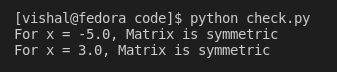
\includegraphics[width=\columnwidth]{./figs/Output.png}
	\caption{Output of Program}
	\label{fig2}
	\end{figure}
\end{enumerate}
\end{document}
